\documentclass{article}
\usepackage[margin=1in]{geometry}
\usepackage{tikz}
\usetikzlibrary{shapes.geometric, arrows, positioning}
%For tikz node diagram setup
\pagenumbering{gobble}

\definecolor{mgreen}{HTML}{689562}
\definecolor{mpurp}{HTML}{85678f}
\definecolor{mblue}{HTML}{3C406C}
\definecolor{mgray}{HTML}{6F6F6F}
\tikzset{trapezium stretches=true}
\tikzstyle{source} = [rectangle, rounded corners, minimum width= 2cm, minimum height = 1cm, text = white, text centered, fill = mgray]
\tikzstyle{input} = [trapezium, trapezium left angle=50, trapezium right angle = 130, minimum width = 1.5cm, minimum height=1cm, text centered, text=white, fill=mgreen]
\tikzstyle{routing} = [diamond, minimum width=2cm, minimum height=1cm, aspect = 2, text width = 2cm, text centered, text=white,fill = mblue]
\tikzstyle{processor} = [rectangle, minimum width = 2cm, minimum height = 1cm, text width = 3cm, text = white, fill = mpurp, text centered]
\tikzstyle{cable} = [thick, ->, >=latex]
\tikzstyle{usb} = [thick, <->, >=latex]


\begin{document}
\centering
\begin{tikzpicture}
\node (bsn) [source] {Bassoon};
\node (lj) [input, right= of bsn] {Little-Jake};
\node (preamp) [routing, right= of lj] {Preamp};
\node (drive) [processor, right= of preamp] {Overdrive};
\node (distortion) [processor, right= of drive] {Distortion};
\node (wah) [processor, right= of distortion] {Auto Wah};
\node (oct) [processor, right= of wah] {Octave};
\node (delay) [processor, right= of oct] {Delay};
\node (chorus) [processor, right= of delay] {Chorus};
\node (verb) [processor, right= of chorus] {Reverb};
\node (amp) [source, right= of verb] {Amp};
\draw [cable] (bsn) -- (lj);
\draw [cable] (lj) -- (preamp);
\draw [cable] (preamp) -- (drive);
\draw [cable] (drive) -- (distortion);
\draw [cable] (distortion) -- (wah);
\draw [cable] (wah) -- (oct);
\draw [cable] (oct) -- (delay);
\draw [cable] (delay) -- (chorus);
\draw [cable] (chorus) -- (verb);
\draw [cable] (verb) -- (amp);
\end{tikzpicture}

\end{document}
